\vspace{-0.25cm}
\section{Introduction}
\label{sec:intro}

Generating efficient code for high performance systems is becoming more and more difficult as these architectures are increasing in complexity and diversity.
Obtaining the best performance requires complex code and data layout transformations, management of complex memory hierarchies, and efficient data communication and synchronization.

For example, consider generalized matrix multiplication (\texttt{gemm}), which computes $C = \alpha AB + \beta C$ and is a
building block of numerous algorithms, including simulations and convolutional neural networks.  Highly-tuned implementations
require fusing the multiplication and addition loops, as well as applying two-level tiling, vectorization, loop unrolling, array packing~\cite{Goto:2008:AHM:1356052.1356053},
register blocking, and data prefetching.  Furthermore, tuned implementations separate partial tiles from full tiles, since partial tiles cannot fully benefit from the same optimizations.
High performance GPU implementations require even more optimizations.  Memory accesses should be coalesced, and data movement must be managed between global memory, shared memory, and registers, with synchronization primitives inserted where necessary.
Automatically generating such complex code is still beyond the capabilities of state-of-the-art compilers.
The importance of kernels such as \texttt{gemm}, along with the immense complexity of optimized implementations, motivate vendors to release highly hand-optimized libraries for such kernels.  However, for most users, obtaining this level of performance for their own code is challenging, since the effort required to explore the space of possible implementations is intractable when hand-coding complex code transformations.

\begin{figure}[t]
\centering
  \begin{minipage}{0.22\textwidth}
    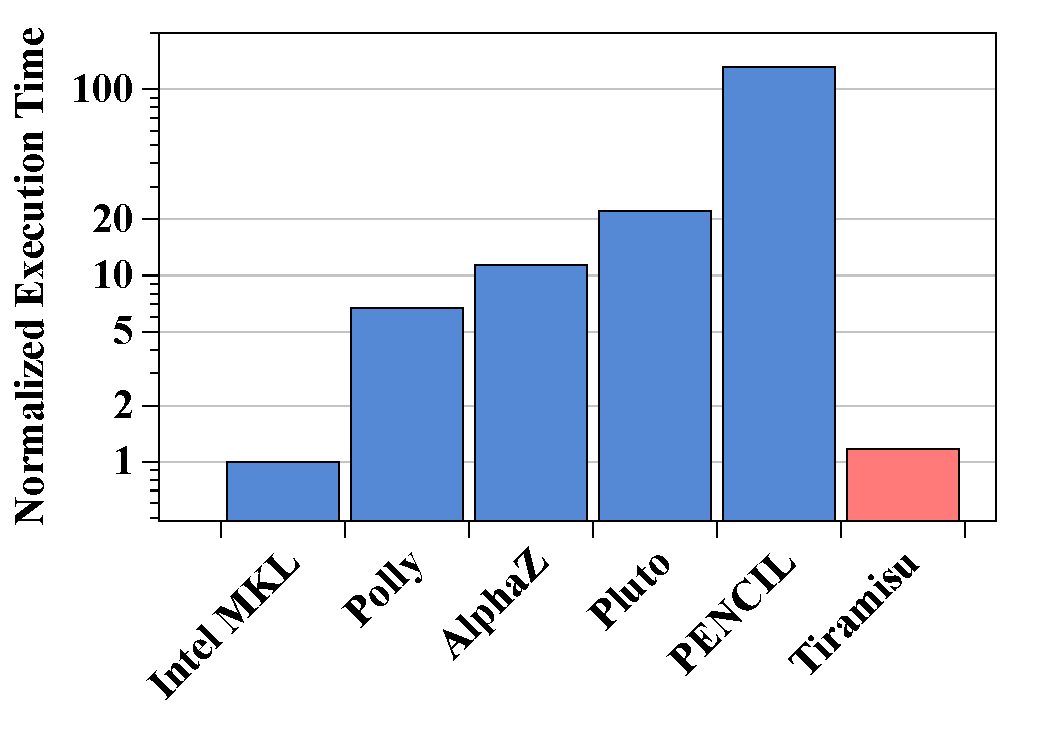
\includegraphics[width=\columnwidth]{./figures/sgemm_performance_CPU.pdf}
  \end{minipage}
  \begin{minipage}{0.22\textwidth}
    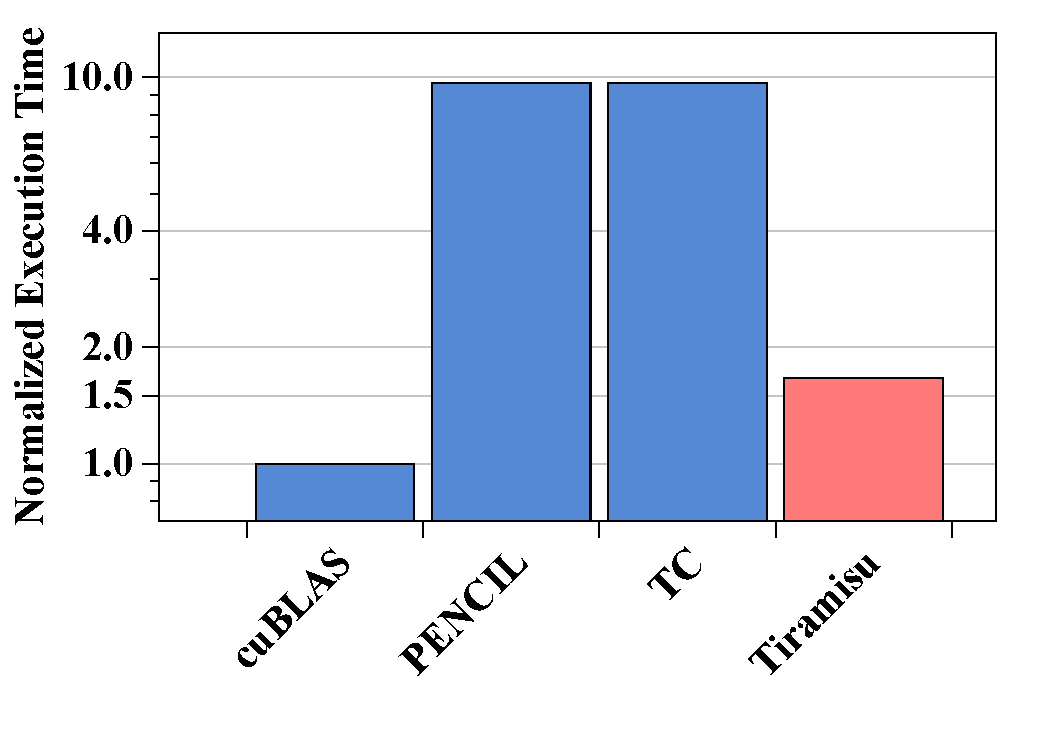
\includegraphics[width=\columnwidth]{./figures/sgemm_performance_GPU.pdf}
  \end{minipage}
  \vspace{-0.5cm}
  \caption{Normalized execution times of code generated for \texttt{sgemm} on CPU (left) and GPU (right).}
  \label{gemm-cpu-gpu}
  \vspace{-0.5cm}
\end{figure}

Previous work with the polyhedral model has shown success in implementing complex iteration space transformations~\cite{wolf1991loop,bondhugula_practical_2008,trifunovic_graphite_2010,polly,Vasilache2018TensorCF}, data locality optimizations~\cite{Iri88,tobias_hexagonal_cgo13}, and memory management optimizations~\cite{feautrier_array_1988,thies_unified_2001,lefebvre_automatic_1998,Qui00,Darte_contraction_2005}.
Although polyhedral compilers are able to represent these program and data transformations and generate complex code, they are still not successful in selecting transformations for the best performance. They still do not match the performance of highly hand-optimized kernels such as \texttt{gemm}. Blue bars in Figure~\ref{gemm-cpu-gpu} show the performance of state-of-the-art polyhedral compilers for \texttt{gemm} compared to the Intel MKL~\cite{mkl} and Nvidia cuBLAS~\cite{cublas} libraries.
Fully-automatic polyhedral compilers such as Polly~\cite{polly}, Pluto~\cite{bondhugula_practical_2008}, and PENCIL~\cite{pencil_paper,pencil_pact}, improve productivity, but fail to obtain the desired level of performance since their search techniques consider only a subset of the necessary optimizations and they rely on less accurate machine models, which leads the compiler to take suboptimal decisions.
Other polyhedral frameworks, such as AlphaZ~\cite{yuki2012alphaz} and CHiLL~\cite{chill}, eschew full automation and instead expose a \textit{scheduling language} that enables users to productively explore the space of possible transformations.
While these frameworks achieve better performance, their scheduling languages are not designed to target GPUs and distributed systems. For example, they do not allow the user to partition computations, send data across nodes, map buffers to GPU shared or local memory,  or insert required synchronization.

In this paper, we introduce \framework{}, the first polyhedral compiler with a scheduling language featuring \emph{novel extensions for targeting multiple high performance architectures}.
\framework{} is well suited for the implementation of data parallel algorithms (loop nests manipulating arrays).
It takes a high level representation of the program (pure algorithm and a set of scheduling commands), applies the necessary code transformations, and generates highly-optimized code for the target architecture.   
In addition to the scheduling commands for loop and data-layout transformations, the \framework{} scheduling language introduces novel commands for computation partitioning, explicit communication and synchronization, and for mapping buffers to different memory hierarchies.
In order to simplify the implementation of the proposed scheduling language, \framework{} explicitly divides the intermediate representation into four-layers that are designed to hide the complexity and large variety of execution platforms by separating the architecture-independent algorithm from the schedule, data-layout, and communication.

%\framework{} differs from prior similar compilers in many respects.  Unlike fully-automatic polyhedral compilers, \framework{} does not rely on machine models and heuristics since these are not always accurate, instead it exposes mechanisms for applying transformations allowing the user to fully control scheduling.  Thanks to this difference, \framework{} can generate more efficient code as shown with the red bars in Figure~\ref{gemm-cpu-gpu}.
The use of a scheduling language has been shown to be an effective method for generating efficient code by multiple compilers including CHiLL, AlphaZ, and Halide~\cite{halide_12,DBLP:conf/pldi/Ragan-KelleyBAPDA13}. Halide is the most successful example as it is now being used in production.
%\framework{} expands existing scheduling languages with a set of novel scheduling commands that allow users to generate more efficient code for a richer set of execution environments, including GPUs, FPGAs, and distributed machines.  Its scheduling language features novel commands for controlling data communication, synchronization and for mapping to different memory hierarchies.
In comparison with Halide in particular, and in addition to the novel extension that \framework{} introduces, \framework{} has an additional fundamental difference: it relies on the expressive polyhedral representation instead of the interval-based representation used by Halide.  This allows \framework{} to express non-rectangular iteration spaces, to support programs with cyclic data-flow graphs, and to apply any affine transformation (including iteration space skewing), all of which are not possible in Halide.

This paper makes the following contributions:

\begin{itemize}
  \item We introduce a polyhedral compiler with a scheduling language that features \emph{novel extensions for controlling data communication, synchronization, and for mapping to different memory hierarchies}.  These extensions enable targeting multiple high-performance architectures including multicore CPUs, GPUs, and distributed machines.

   % We explicitly divide the IR into 4 layers to simplify the implementation ...
  \item We explicitly divide the intermediate representation into four-layers to simplify the implementation of the proposed scheduling language.  The four-layers IR separates the algorithm from code transformations and data-layout transformations, allowing for portability and simplifying the composition of architecture-specific lowering transformations.

  \item We evaluate \framework{} on a set of image processing and stencil benchmarks and compare it with Halide, an industrial compiler with a scheduling language, and with PENCIL, a state-of-the-art polyhedral compiler.  We show that Tiramisu matches or outperforms existing compilers on different hardware architectures, including multicore CPUs, GPUs, and distributed machines.
\end{itemize}

%TODO: unify scheduling language term.
